\documentclass{beamer}
\usepackage[T2A]{fontenc}
\usepackage[utf8]{inputenc}
\usepackage[english,russian]{babel}
\usepackage{amssymb,amsfonts,amsmath,mathtext}
\usepackage{cite,enumerate,float,indentfirst}
\usepackage{multirow}
\usepackage{array}
\usepackage{comment} %подключение комментариев
%\usetheme{Dresden}

% Для исходного кода:
\usepackage{color} 
\usepackage{listings} 

\usetheme{Warsaw}
\setbeamercovered{dynamic}

\title[]%
{Статический анализ кода пакетов прикладных программ для поиска протяженных
        участков для замены на параллельный эквивалент}
\author[А.Н.~Сальников, М.В.~Чернова]
{
    \underline{А.Н.~Сальников}\textsuperscript{1,2},
               М.В.~Чернова\textsuperscript{1}
}

\institute{
             ВМК МГУ имени М.В. Ломоносова\textsuperscript{1},\newline
             ФИЦ ИУ РАН\textsuperscript{2},\newline
}

   \date{}

\begin{document}

\lstset {
language = C,
basicstyle=\small\sffamily,
showspaces=false,  
showstringspaces=false,
tabsize=2, 
escapeinside={\%*}{*)} 
}

\begin{frame}
	\titlepage
\end{frame}




\begin{frame}
\frametitle{Введение}
\begin{itemize}
	\item В научной среде существует множество пакетов прикладных
программ (ППП), активно использующихся в решении различных
задач.
	\item Ежегодная разработка новых программных продуктов вызывает
устаревание некоторых программных решений, в частности
отдельных частей в пакетах прикладных программ.
	\item Возникает вопрос о повышении эффективности работы такого
кода, а также о различных его модификациях с минимизацией
затрат человеческого труда.
\end{itemize}
\end{frame}

\begin{frame}
\frametitle{Идея работы}
\begin{itemize}
	\item Создание системы выдачи рекомендаций пользователю о возможности замены
	 некоторых фрагментов в пакете прикладных программ с целью дальнейшей оптимизации
\end{itemize}

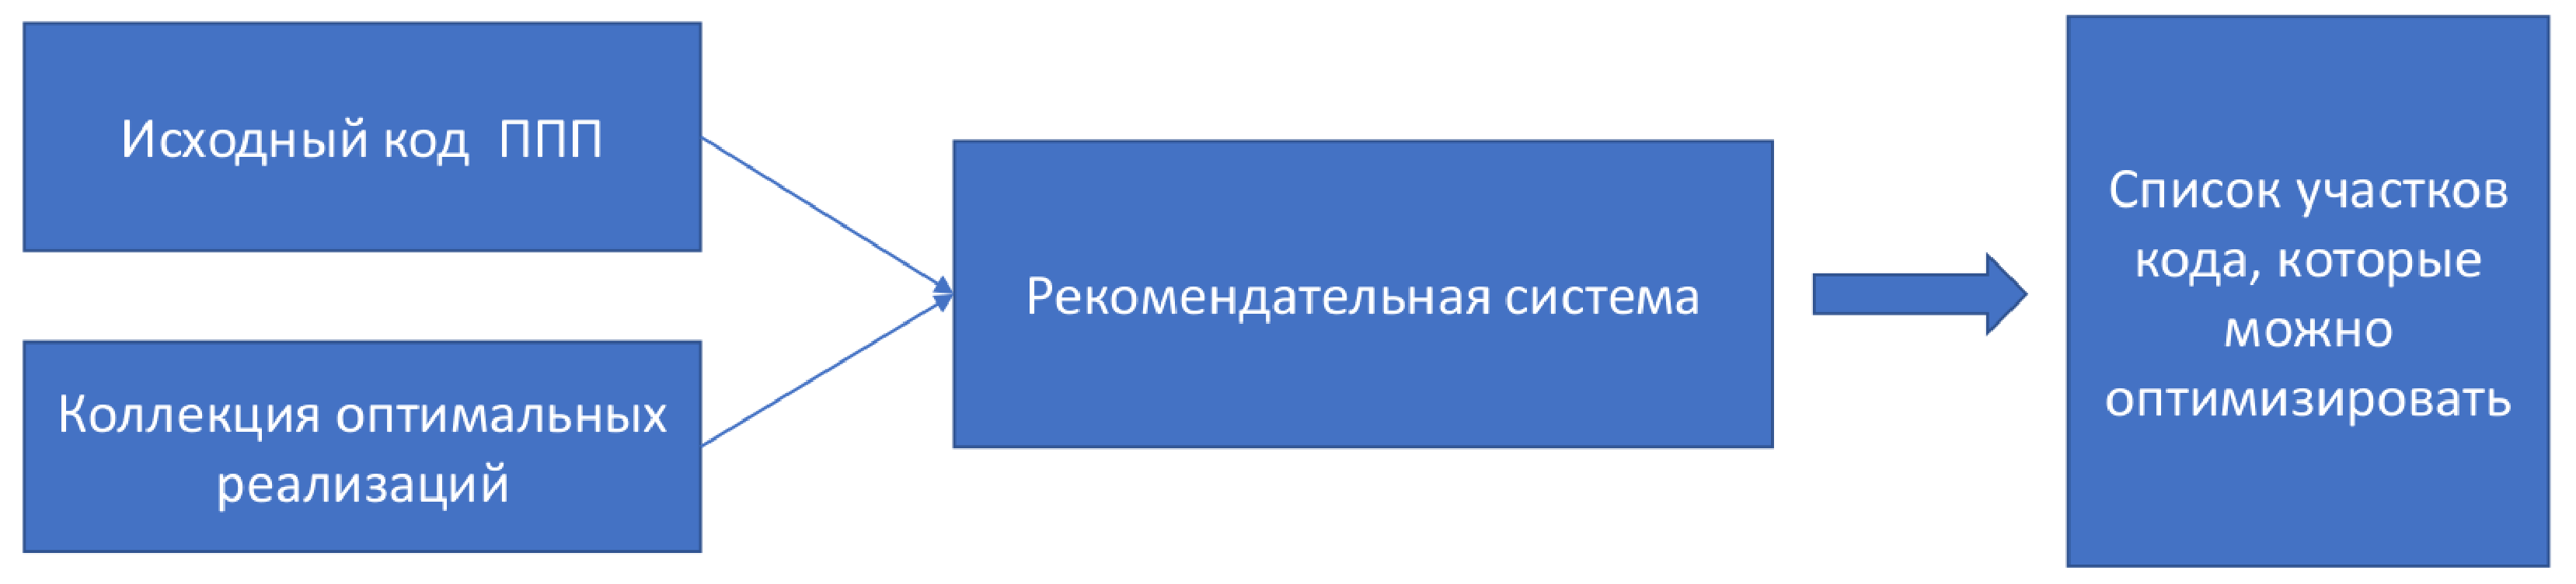
\includegraphics[width=\textwidth]{img/idea.eps}
\end{frame}

\begin{frame}
\frametitle{Подзадачи}
\begin{itemize}
	\item Создание коллекции реализаций часто используемых в ППП численных методов
	\item Создание метода поиска в исходном коде фрагментов, функционально
	 эквивалентных заданному
	\item Создание коллекции целевых фрагментов с учетом различных характеристик
	 «оптимальности». Под «оптимальностью» будем иметь в виду реализацию в
	  соответствии с запросами пользователя (например, для конкретного окружения)
\end{itemize}
\end{frame}

\begin{frame}
\frametitle{Цели и трудности решения}
Цели: 
\begin{itemize}
	\item Найти в исходном коде ППП расположение фрагментов кода, функционально
эквивалентных данному.
	\item Иметь возможность находить не только фрагменты, идентичные искомому, но
также имеющие расхождения по различному ряду признаков, таких как: имена
переменных/функций, порядок расположения операторов, наличие или
отсутствие некоторых операторов.
\end{itemize}

Трудности решения: 
\begin{itemize}
	\item Большой объем исходного кода, в котором должен производиться поиск
(следовательно, трудность построения графа потока управления).
	\item Нет однозначности при определении функциональной эквивалентности двух
участков кода.
\end{itemize}
\end{frame}

\begin{frame}
\frametitle{Описание предлагаемого подхода}
\begin{itemize}
	\item Создание базы фрагментов кода, на основании которой будет производиться поиск.
	\item Создание базы оптимальных функциональных эквивалентов для предложения замены найденных фрагментов.
	\item Осуществление поиска схожих фрагментов по созданной базе в каком-либо пакете
прикладных программ.
\end{itemize}
\end{frame}

\begin{frame}
\frametitle{Рассматриваемые ППП}
\begin{itemize}
	\item OpenFOAM  ---
	 открытое программное обеспечение для численного моделирования задач механики
	 сплошных сред. В основе кода лежит набор библиотек, предоставляющих инструменты
	 для решения систем дифференциальных уравнений в частных производных. 
\end{itemize}
\begin{center}
\includegraphics[width=0.7\textwidth]{img/openfoam.eps}
\end{center}
\end{frame}


\begin{frame}
\frametitle{Рассматриваемые ППП}
\begin{itemize}
	\item Gromacs  --- (groningen machine for chemical
simulations --- гронингенская машина для химического моделирования) --- пакет
 программдля моделирования физико-химических процессов в молекулярной динамике,
  специализирующийся на моделировании биомолекул (например, молекул белков и липидов),
   имеющих много связанных взаимодействий между атомами.
\end{itemize}
\end{frame}

\begin{frame}
\frametitle{Рассматриваемые ППП}
\begin{itemize}
	\item MPIESM(ECHAM6/MPIOM/JSBACH/HAMOCC) --- современная крупномасштабная
    совместная модель <<океан-земля-атмосфера>> европейского метеорологического сообщества.
\end{itemize}
\begin{center}
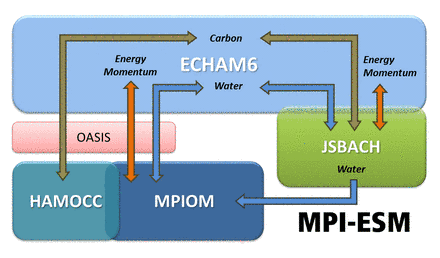
\includegraphics[width=0.7\textwidth]{img/mpiesm.png}
\end{center}
\end{frame}

\begin{frame}
\frametitle{Характеристики пакетов прикладных программ}
\renewcommand{\arraystretch}{1.8} %% increase table row spacing
%\renewcommand{\tabcolsep}{0.3cm} 
\begin{tabular}{|p{3.8cm}|c|c|c|}
\hline
 & OpenFOAM &  Gromacs & MPI-ESM\\
\hline
Общее количество
\newline файлов & 15,639 & 4,563 & 3,990\\
\hline
Общее количество строк & 4,517,786 & 3,006,701 & 4,034,054 \\
\hline
Количество строк  кода
\newline в файлах типа .c, .f* & 1,626,725 & 2,246,960 & 1,018,752\\
\hline
\end{tabular}
\end{frame}

\begin{frame}
\frametitle{Создание базы исходного кода для поиска}
В качестве искомых мотивов будут использованы реализации математических методов,
 однако сам алгоритм может быть использован и для других методов. 

В качестве реализаций математических методов было принято решение использовать
 следующие библиотеки: 
\begin{itemize}
	\item ATLAS(Automatically Tuned Linear Algebra Software) -- реализация BLAS для
	 языков C и Fortran. Средний объем методов 268 строк.
	\item OpenCV (Open Source Computer Vision Library) -- библиотека алгоритмов
	 компьютерного зрения, обработки изображений и численных алгоритмов общего
	  назначения  для языка С. Средний объем методов 297 строк.
\end{itemize}
\end{frame}

\begin{frame}
\frametitle{Построение решения для поиска схожих фрагментов}
\begin{itemize}
	\item Создание списка зависимостей, требуемых мотивом.
	\item Обнаружение рекурсий.
	\item Генерация нового файла, включающего все необходимые вызовы процедур.
	\item Удаление незначащих фрагментов.
\end{itemize}
\end{frame}

\begin{frame}
\frametitle{Предобработка исходного кода пакета прикладных программ}
\begin{itemize}
	\item Анализ пакета: обнаружение и составление списка файлов реализации на
	 конкретном языке.
	\item Кластеризация файлов: отобранные файлы разбиваются на множество кластеров
по наличию зависимостей для поэтапного сравнения с шаблоном.
	\item Удаление комментариев: до кластеризации или после,
отдельно для каждого кластера.
\end{itemize}
\end{frame}



\begin{frame}
\frametitle{Создание комплексной метрики для определения близости фрагментов}
\begin{enumerate}
	\item Фрагментом кода в заданном файле $f$ будем считать последовательность лексем $L_i$, однозначно определяемую парой $\langle l_{begin}, l_{end}\rangle$, где $l_{begin}$ и $l_{end}$ -- номера строк начала и конца фрагмента соответственно.
	
	\item $\mathcal{P} = \{\mathcal{P}_i | 1 \leq i \leq N_p \}$ -- множество  исходного кода в пакете прикладной программы, 
	
	\item $ M = \{M_j | 1 \leq j \leq N_m \}$ -- множество реализаций из коллекции искомых фрагментов.	
	
	\item Тогда для двух фрагментов $L_{\mathcal{P}_i}$ и $L_{M_j}$ зададим функцию $\rho (L_{\mathcal{P}_i}, L_{M_j})$ -- расстояние между ними.
	\item Фрагмент $L_{\mathcal{P}_i}$ будем называть дубликатом фрагмента $L_{M_j}$ в отношении $ \varphi$, если $\rho (L_{\mathcal{P}_i}, L_{M_j}) \leq \varphi \leq 1$.
\end{enumerate}
\end{frame}


\begin{frame}
\frametitle{Реализация алгоритма с использованием выбранных метрик}
\begin{itemize}
	\item На данном этапе был выбран способ вычисления метрики схожести на основании  абстрактных синтаксических деревьев\footnote[1]{Baxter I. D. et al. Clone detection using abstract syntax trees}:
\begin{equation}
S ~ (L_{\mathcal{P}_i}, M_j) = \frac{2 N}{2 N + L + R},
\end{equation}
где $N$ — число совпадающих узлов, $L$ — число различных узлов в первом поддереве, $R$ — число различных узлов во втором поддереве.
	\item Построение деревьев производилось с помощью генератора парсеров ANTLR.
\end{itemize}

\end{frame}



\begin{frame}
\frametitle{Результаты работы}
\begin{itemize}
	\item При кластеризации использовалась глубина, равная 3.
	\item Время указано в секундах	
\end{itemize}
\begin{small}	
\renewcommand{\arraystretch}{1.2} %% increase table row spacing
\renewcommand{\tabcolsep}{0.3cm} 
\begin{tabular}{|p{3.8cm}|c|c|c|}
\hline
 & OpenFOAM &  Gromacs & MPI-ESM\\
\hline
Время анализа файлов & 3.06 & 0.815 & 0.862\\
\hline
Количество \newline обработанных файлов & 8336 & 3206 & 1884 \\
\hline
Время кластеризации  & 203.475 & 93.467 & 53.48\\
\hline
Количество кластеров & 3643 & 2484 & 1167\\
\hline
Время \newline удаления комментариев & 257.103 & 121.467 & 85.225\\
\hline
Количество удаленных строк & 15975 & 5775 & 5280\\
\hline
\end{tabular}
\end{small}
\end{frame}

\begin{frame}
\frametitle{Результаты работы}
\begin{itemize}
	\item Описанный алгоритм поиска фрагментов был применен на пакете MPI-ESM. В
качестве базы, на основании которой производился поиск, была создана коллекция реализаций численных методов, наиболее часто встречающихся в пакете
	\item Поиск осуществлялся при пороговом значении метрики 0.7
\end{itemize}
\end{frame}

\begin{frame}
\frametitle{Количество найденных функций}
\begin{small}
\begin{center}
\renewcommand{\arraystretch}{1.8} %% increase table row spacing
%\renewcommand{\tabcolsep}{0.3cm} 
\begin{tabular}{|p{1.6cm}|p{1.4cm}|p{1.0cm}|p{1.3cm}|p{1.5cm}|p{1.9cm}|}
\hline
 & Метод Ньютона &  Метод Гаусса & Метод релаксации & Метод простой итерации & Метод Ричардсона\\
\hline
Вызовы 
\newline функций & 5 & 11 & 2 & 6 & 5 \\
\hline
Схожие 
\newline реализации & 12 & 28 & 15 & 8 & 3\\
\hline
\end{tabular}
\end{center}
\end{small}
\end{frame}

\begin{frame}
\frametitle{Дальнейшая работа}
\begin{itemize}
	\item[\textbullet] Создание базы шаблонов параллельных реализаций некоторых методов, которые будут предложены пользователю в качестве замены 
	\item[\textbullet] Реализация алгоритма выдачи информации о всех найденных схожих шаблонах и рекомендаций о замене и подстановке оптимальных эквивалентов	
	\item[\textbullet] Рассмотреть возможность интеграции такой системы в системы автоматического распараллеливания кода
\end{itemize}
\end{frame}




\lstset{
language=C++,
basicstyle=\tiny\sffamily,
numbers=left,
numberstyle=\tiny, 
numbersep=5pt,                % как далеко отстоят номера строк от подсвечиваемого кода
showstringspaces=false,      % показывать или нет пробелы в строках
showtabs=false,             % показывать или нет табуляцию в строках
tabsize=2,                 % размер табуляции по умолчанию равен 2 пробелам
breaklines=true,           % автоматически переносить строки (да\нет)
breakatwhitespace=false, % переносить строки только если есть пробел
escapeinside={\%*}{*)}   % если нужно добавить комментарии в коде
}






\begin{frame}
\begin{center}
	Спасибо за внимание!
\end{center}
\end{frame}



\begin{frame}
\frametitle{Терминология}
\begin{itemize}
	\item \textit{Дубликаты} -- два функционально эквивалентных фрагмента кода.
	\item Под \textit{методом} будет подразумеваться один из алгоритмических способов решения конкретной задачи.
	\item Каждый метод может иметь несколько \textit{мотивов} – конкретных вариантов реализации, которые разрабатываются в зависимости от возможностей вычислительной системы и алгоритма, используемого разработчиком.
	\item \textit{Код пакета прикладных программ} (код ППП) – реализация пакета прикладных про-
грамм, в которой необходимо обнаружить дубликат искомого мотива.
	\item \textit{Шаблон} -- искомый мотив, по которому непосредственно будет осуществляться поиск в коде ППП.
\end{itemize}
\end{frame}




\end{document}

%\documentclass[fullscreen=true, bookmarks=false]{beamer}
%\usepackage[utf8]{inputenc}
%\usepackage[english,russian]{babel}
%\usepackage{xcolor}
%\usetheme{Dresden}
